% Provenance (never printed): cycle 4 SVT, "La planete Terre, l'environnement
% et l'action humaine": natural risks, hazard and vulnerability, prevention
% and protection; see sources/book1/PROVENANCE.md. Book 1, grade 9, chapter 2.
% Vocabulary guard: owns risk, vulnerability, prevention, hazard map.
% Natural hazard and natural disaster, the warning colours and the safety
% rules are g5's (natural-hazards); the warning signs of an eruption and the
% Pinatubo story are g7's (volcanoes); seismometer, tsunami and "scientists
% cannot predict earthquakes" are g7's (earthquakes); flood and floodplain
% are g5's (water-shapes-the-land); weather forecast is g8's. Lahars are
% called mudflows (as in g7). "Normal fault" is Book 2's: here "a fault".
\chapter{与自然风险共存}\label{ch:g9:natural-risks}

1985 年 11 月 13 日深夜，哥伦比亚阿尔梅罗镇的大多数人
已经入睡。一场\omterm{def:g5:natural-hazards:storm}{风暴}遮住了覆雪的内瓦多
德鲁伊斯\omterm{def:g4:volcanoes-earthquakes-first-look:volcano}{火山}，距小镇 \qty{45}{km}，镇上无人看见它\omterm{def:g4:volcanoes-earthquakes-first-look:eruption}{喷发}。炽热的
岩块融化了部分冰雪，融水与\omterm{def:g4:volcanoes-earthquakes-first-look:eruption}{火山灰}和岩屑混合，
沿\omterm{def:g1:landscapes-around-us:landform}{山谷}冲下，形成泥石流。约两小时后，泥石流
从拉古尼利亚斯河的河谷倾泻而出，直冲小镇：
约 \num{23000} 人遇难，占全镇大部分人口。两小时
足以走到更高的地方。阿尔梅罗的居民未得到任何通知。
% ledger: usgs:armero

\begin{omfigure}
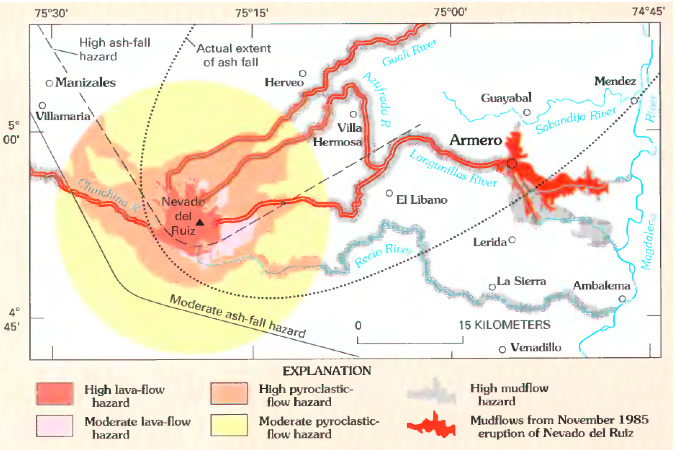
\includegraphics[width=0.86\linewidth]{images/book1/g9-ruiz-hazard-map.jpg}

{\small 内瓦多德鲁伊斯\omterm{def:g4:volcanoes-earthquakes-first-look:volcano}{火山}\omterm{def:g9:natural-risks:hazard-map}{危害分布图}。最初一版由哥伦比亚地质学家绘制，
在\omterm{def:g4:volcanoes-earthquakes-first-look:eruption}{喷发}前一个月流传，
已指出阿尔梅罗河谷中泥石流的危险。本图
为灾后重绘，用亮红色标出 1985 年 11 月真正袭来的泥石流
确于 1985 年 11 月发生（\omterm{def:g4:volcanoes-earthquakes-first-look:volcano}{火山}周围阴影圆的半径约为
\qty{20}{km}）。出处：T.~L.~赖特与T.~C.~皮尔森，USGS
Circular 1073，1992（公有领域，经维基共享资源）。}
% ledger: usgs:ruiz-map, commons:ruiz-map
\label{fig:g9:natural-risks:ruiz}
\end{omfigure}

六年后，在菲律宾的皮纳图博\omterm{def:g4:volcanoes-earthquakes-first-look:volcano}{火山}，\omterm{def:g4:volcanoes-earthquakes-first-look:volcano}{火山}正被
持续监测，预警及时发出，居民得以撤离
（见\cref{ch:g7:volcanoes}）。两者都是爆发式\omterm{def:g4:volcanoes-earthquakes-first-look:volcano}{火山}，
两者的泥石流路径上都有人居住。二者的不同在于人们
知道什么，以及如何利用这些知识。本章
讨论的正是这一区别。
% ledger: usgs:armero (Pinatubo 1991 averted a disaster like Armero), usgs:pinatubo-1991

\begin{recall}
可能伤害人类的自然事件称为\emph{\omterm{def:g5:natural-hazards:hazard}{自然危害}}；它
若发生于人类居住之地，并造成重大伤害，便成为\emph{\omterm{def:g5:natural-hazards:disaster}{自然灾害}}
（见\cref{ch:g5:natural-hazards}）。泛滥的\omterm{def:g1:landscapes-around-us:water}{河流}
会淹没其\omterm{def:g5:water-shapes-the-land:flood}{河漫滩}（见\cref{ch:g5:water-shapes-the-land}）。\omterm{def:g4:volcanoes-earthquakes-first-look:volcano}{火山}
在大规模\omterm{def:g4:volcanoes-earthquakes-first-look:eruption}{喷发}前常有预兆：小\omterm{def:g4:volcanoes-earthquakes-first-look:earthquake}{地震}、
山坡隆起、气体释放（见\cref{ch:g7:volcanoes}）。科学家无法预测
\omterm{def:g4:volcanoes-earthquakes-first-look:earthquake}{地震}；\omterm{def:g7:earthquakes:seismometer}{地震仪}记录\omterm{def:g4:volcanoes-earthquakes-first-look:earthquake}{地震}，海底\omterm{def:g4:volcanoes-earthquakes-first-look:earthquake}{地震}
可引发\omterm{def:g7:earthquakes:tsunami}{海啸}（见\cref{ch:g7:earthquakes}）。\omterm{def:g8:fronts-and-weather-maps:forecast}{天气预报}
用于说明未来几天的\omterm{def:g1:watching-the-weather:weather}{天气}状况
（见\cref{ch:g8:fronts-and-weather-maps}）。
\end{recall}

\section{危害、脆弱性与风险}

同样的\omterm{def:g4:volcanoes-earthquakes-first-look:earthquake}{地震}并非处处造成相同的损害。在一片空旷的
\omterm{def:g5:weather-and-climate:desert}{沙漠}中，它不伤害任何人。在建筑坚固、居民
知道如何应对的城镇中，它只会造成震动、惊吓和玻璃破碎；在
房屋笨重、建造粗劣的城镇中，它可能使房屋倒塌，压住屋内的人。
危害本身相同；变化的是这个地方
受到伤害的难易程度。

\begin{definition}[脆弱性]\label{def:g9:natural-risks:vulnerability}
某地的\emph{脆弱性}\index{脆弱性}是指
其人口、建筑及生活所需之物易受\omterm{def:g5:natural-hazards:hazard}{自然危害}伤害的程度。
\omterm{def:g5:water-shapes-the-land:flood}{河漫滩}上的住房、结构薄弱的建筑、无预警且无规划，
都会使某地变得脆弱。
\end{definition}

\begin{definition}[风险]\label{def:g9:natural-risks:risk}
某地面临\omterm{def:g5:natural-hazards:hazard}{自然危害}时的\emph{风险}\index{风险}是
其人员与财物遭受伤害的危险程度。它既取决于
危害的强度与频率，也取决于该地的
\omterm{def:g9:natural-risks:vulnerability}{脆弱性}：若无危害，或无可受损之物，则
便不存在风险。
\end{definition}

\begin{omfigure}
\begin{tikzpicture}[x=1cm, y=1cm, font=\footnotesize,
    cell/.style={minimum width=4.6cm, minimum height=2.2cm, align=center, draw=black!50, text width=4.2cm}]
  \node[cell, fill=green!25] at (2.3,1.1) {\textbf{低风险}\\ 无人居住的山谷中的小洪水};
  \node[cell, fill=orange!30] at (6.9,1.1) {\textbf{中等风险}\\ 强震下的 \\ 建筑坚固、居民有准备的城镇};
  \node[cell, fill=orange!30] at (2.3,3.3) {\textbf{中等风险}\\ 河漫滩上的村庄 \\ 遭遇小洪水};
  \node[cell, fill=red!35] at (6.9,3.3) {\textbf{高风险}\\ 强震下的 \\ 建筑薄弱、无规划的城镇};
  \draw[->, thick] (0,-0.25) -- (9.4,-0.25);
  \draw[->, thick] (-0.25,0) -- (-0.25,4.6);
  \node[anchor=north] at (4.6,-0.7) {危害（更强、更频繁）$\longrightarrow$};
  \node[rotate=90, anchor=south] at (-1.0,2.2) {脆弱性 $\longrightarrow$};
  \node[below] at (2.3,-0.25) {低};
  \node[below] at (6.9,-0.25) {高};
  \node[left] at (-0.25,1.1) {低};
  \node[left] at (-0.25,3.3) {高};
\end{tikzpicture}

{\small \omterm{def:g9:natural-risks:risk}{风险}网格（示意图）。\omterm{def:g9:natural-risks:risk}{风险}随危害与
\omterm{def:g9:natural-risks:vulnerability}{脆弱性}的增大而增大。迁移城镇很少可行，危害
也无法消除；但可以降低其\omterm{def:g9:natural-risks:vulnerability}{脆弱性}，
从而使城镇在网格中向下移动。}
\label{fig:g9:natural-risks:grid}
\end{omfigure}

阿尔梅罗是高危害之地：一座覆雪的\omterm{def:g4:volcanoes-earthquakes-first-look:volcano}{火山}在一年前苏醒，
小镇建在古老泥石流的堆积物上，位于
曾经输送过泥石流的\omterm{def:g1:landscapes-around-us:landform}{山谷}谷口。阿尔梅罗还
极为脆弱：科学家缺乏仪器与支持，
向当局提供的信息往往含糊不清，没有
疏散计划，也没有迅速通知全镇的办法。
% ledger: usgs:armero

\section{预报与预防}

有些危害是可以提前看到的。\omterm{def:g5:natural-hazards:storm}{风暴}可提前数天预报
（见\cref{ch:g8:fronts-and-weather-maps}）；强降雨后的\omterm{def:g5:water-shapes-the-land:flood}{洪水}可提前数小时至数天预报；
大规模\omterm{def:g4:volcanoes-earthquakes-first-look:eruption}{喷发}通常会提前数天至数周显露迹象，
但并非总是如此。\omterm{def:g7:earthquakes:tsunami}{海啸}横跨大洋只需数小时，因此
预警可以先于\omterm{def:g7:earthquakes:tsunami}{海啸}抵达遥远\omterm{def:g1:landscapes-around-us:water}{海岸}。另一方面，\omterm{def:g4:volcanoes-earthquakes-first-look:earthquake}{地震}无法预测：
科学家可以说出哪些\omterm{def:g7:earthquakes:fault}{断层}终将再次断裂，
却永远无法说出具体哪一天。
% ledger: nws:tsunami-speed, usgs:eq-basics, usgs:pinatubo-1991

预报无论多么准确，只有在危害来袭之前采取行动，才有用。
这些工作大多在任何预警发出之前很久就已完成。

\begin{definition}[预防]\label{def:g9:natural-risks:prevention}
\emph{预防}\index{预防}是指在\omterm{def:g5:natural-hazards:hazard}{自然危害}来袭之前为降低\omterm{def:g9:natural-risks:risk}{风险}而做的一切工作：
了解危害可能发生的地点，
在安全地点以安全方式建设，监测危害，
向民众发出预警并使其做好准备。
\end{definition}

\omterm{def:g9:natural-risks:prevention}{预防}在\omterm{def:g9:natural-risks:risk}{风险}网格的两个方面都起作用。观测\omterm{def:g4:volcanoes-earthquakes-first-look:volcano}{火山}或\omterm{def:g1:landscapes-around-us:water}{河流}
并不会降低其危险，但能争取到行动的时间。在远离\omterm{def:g5:water-shapes-the-land:flood}{河漫滩}的地方建房、
建造坚固的房屋、规划通往高地的路线并加以演练，
都能降低\omterm{def:g9:natural-risks:vulnerability}{脆弱性}。

\begin{omfigure}
\begin{minipage}[c]{0.44\linewidth}\centering

\includegraphics[width=\linewidth]{images/book1/ai/g9-emergency-kit.jpg}
\end{minipage}\hfill
\begin{minipage}[c]{0.52\linewidth}\raggedright
{\small 做好准备：一家人检查放在门边的应急包，
以便在必须迅速离开时随手带走：可保存数天的水和食物，
手电筒、不依赖市电的收音机，
备用电池、急救包和保暖毯。
（AI 生成的通用场景示意图）。}
\end{minipage}
% ledger: ready:kit
\label{fig:g9:natural-risks:kit}
\end{omfigure}

\section{监测火山与断层}

\omterm{def:g4:volcanoes-earthquakes-first-look:volcano}{火山}观测站监测\cref{ch:g7:volcanoes}中的预警信号，
借助昼夜不停运行的仪器，
并将读数传回观测站。
% ledger: usgs:hvo-toolkit

\begin{omfigure}
\begin{tikzpicture}[x=1cm, y=1cm, font=\footnotesize, >={Stealth[length=2mm]}]
  % ground and cone
  \fill[black!13] (0,0) -- (0,1.0) -- (3.0,1.2) -- (5.4,3.6) -- (6.4,3.6) -- (8.8,1.2) -- (12,1.0) -- (12,0) -- cycle;
  \draw[black!60] (0,1.0) -- (3.0,1.2) -- (5.4,3.6) -- (6.4,3.6) -- (8.8,1.2) -- (12,1.0);
  % magma chamber and conduit
  \fill[omWarm!70] (5.9,0.6) ellipse (1.5 and 0.38);
  \fill[omWarm!70] (5.75,0.9) rectangle (6.05,3.6);
  \node[white, font=\scriptsize\bfseries] at (5.9,0.58) {岩浆};
  % gas plume, drifting west
  \fill[black!10] (5.8,3.95) circle (0.3) (5.35,4.35) circle (0.4) (4.75,4.75) circle (0.45);
  % swollen east flank, dashed
  \draw[dashed, omWarm, line width=0.8pt] (6.45,3.7) .. controls (7.5,3.55) and (8.6,2.6) .. (8.85,1.25);
  \draw[->, omWarm] (7.3,2.75) -- (7.7,3.15);
  \node[anchor=west, align=left, text=omWarm!80!black] at (8.2,3.75) {上升的岩浆 \\ 使斜坡隆起};
  % tiltmeter on the east flank
  \fill[black] (7.75,2.12) rectangle (8.05,2.24);
  \draw[black!70] (8.1,2.2) -- (8.5,2.45);
  \node[anchor=west, align=left] at (8.5,2.55) {倾斜仪：斜坡 \\ 随隆起而倾斜};
  % GPS receiver on the west flank, and its satellite
  \draw[black, line width=0.6pt] (4.4,2.6) -- (4.4,2.95);
  \fill[black] (4.25,2.95) rectangle (4.55,3.05);
  \draw[black] (4.4,3.05) circle (0.1);
  \draw[black, fill=white] (1.7,4.85) rectangle (2.0,5.05);
  \draw[black] (1.4,4.95) -- (2.3,4.95);
  \node[anchor=east] at (1.35,4.95) {卫星};
  \draw[black!50, dashed] (4.3,3.15) -- (2.05,4.8);
  \draw[black!70] (3.05,2.65) -- (4.2,2.85);
  \node[anchor=east, align=right] at (3.0,2.6) {GPS 接收器：\\ 地面移动 \\ 以毫米计};
  % gas instrument on the crater rim
  \fill[black] (6.45,3.6) rectangle (6.75,3.75);
  \draw[black!70] (6.8,3.75) -- (7.1,4.45);
  \node[anchor=west, align=left] at (7.1,4.6) {气体探测仪：\\ 测量从火山口 \\ 逸出的气体};
  % seismometer (in the ground)
  \fill[black] (2.1,0.95) rectangle (2.4,1.1);
  \node[anchor=north, align=center] at (1.6,0.85) {地震仪：\\ 记录小地震};
  % camera, east, looking at the summit
  \fill[black] (10.7,1.12) rectangle (11.0,1.32);
  \fill[black] (10.7,1.17) -- (10.55,1.12) -- (10.55,1.32) -- (10.7,1.27) -- cycle;
  \node[anchor=north, align=center] at (10.8,0.85) {照相机：\\ 监视山顶};
\end{tikzpicture}

{\small \omterm{def:g4:volcanoes-earthquakes-first-look:volcano}{火山}监测示意图（非按比例绘制）。\omterm{def:g7:earthquakes:seismometer}{地震仪}统计
小\omterm{def:g4:volcanoes-earthquakes-first-look:earthquake}{地震}；倾斜仪和 GPS 接收器固定在\omterm{def:g3:stones-pebbles-sand:rock}{岩石}上，
测量\omterm{def:g7:volcanoes:magma}{岩浆}在地下聚集时地面如何倾斜和移动；
其他仪器测量逸出的气体；照相机监视
山顶。\omterm{def:g4:clouds-rain-snow:rain-gauge}{雨量计}有助于区分\omterm{def:g4:volcanoes-earthquakes-first-look:volcano}{火山}信号与
强降雨的影响。}
% ledger: usgs:hvo-toolkit
\label{fig:g9:natural-risks:monitoring}
\end{omfigure}

这些迹象都无法给出\omterm{def:g4:volcanoes-earthquakes-first-look:eruption}{喷发}的具体日期和时刻。科学家
把它们综合起来解读，如同医生综合分析病人的多项检查，
并判断危险如何变化；当局则决定何时封闭某一区域、何时组织人员撤离。
在皮纳图博\omterm{def:g4:volcanoes-earthquakes-first-look:volcano}{火山}，这一链条运作良好。在鲁伊斯\omterm{def:g4:volcanoes-earthquakes-first-look:volcano}{火山}，
\omterm{def:g4:volcanoes-earthquakes-first-look:volcano}{火山}已持续一年发出迹象，
伴有震群，但仪器稀少，从科学家到阿尔梅罗民众
的信息链条断裂了。
% ledger: usgs:armero, usgs:hvo-toolkit, usgs:pinatubo-1991

\omterm{def:g7:earthquakes:fault}{断层}的监测方式与此类似，即通过\omterm{def:g7:earthquakes:seismometer}{地震仪}网络和
GPS 观测站网络，逐毫米测量\omterm{def:g7:earthquakes:fault}{断层}的两侧
如何缓慢移动。这可以指出哪些\omterm{def:g7:earthquakes:fault}{断层}正在积累
下一次强震的应变，但无法得知何时发生。对于
\omterm{def:g4:volcanoes-earthquakes-first-look:earthquake}{地震}而言，\omterm{def:g9:natural-risks:prevention}{预防}是最主要的防御手段。
% ledger: usgs:gps, usgs:eq-basics

\section{洪水与泛洪区图}

防灾的第一步，是知道危害可能在何处发生。

\begin{definition}[危害分布图]\label{def:g9:natural-risks:hazard-map}
\emph{危害分布图}\index{危害分布图}标示出\omterm{def:g5:natural-hazards:hazard}{自然危害}可能波及的地点，
其中常包含若干危险等级。
绘制依据是危害过去造成的后果，以及地面的形状。
\end{definition}

本章开头的内瓦多德鲁伊斯\omterm{def:g4:volcanoes-earthquakes-first-look:volcano}{火山}图即是一幅\omterm{def:g9:natural-risks:hazard-map}{危害分布图}：
过去的泥流沿\omterm{def:g1:landscapes-around-us:landform}{山谷}流动，下一次泥流也很可能沿同样的\omterm{def:g1:landscapes-around-us:landform}{山谷}流动。
\omterm{def:g5:water-shapes-the-land:flood}{洪水}图遵循相同的思路。\omterm{def:g1:landscapes-around-us:water}{河流}两侧低平的地面
会被\omterm{def:g5:water-shapes-the-land:flood}{洪水}淹没，\omterm{def:g5:water-shapes-the-land:flood}{洪水}越高，淹没的范围越宽。
\omterm{def:g5:water-shapes-the-land:flood}{洪水}图画出的是某一设定\omterm{def:g5:water-shapes-the-land:flood}{洪水}的水边界，
通常取每年有 1/100 的概率达到或超过的那一\omterm{def:g5:water-shapes-the-land:flood}{洪水}，
它被称为
\emph{百年一遇\omterm{def:g5:water-shapes-the-land:flood}{洪水}}，但它并非每百年才来一次的\omterm{def:g5:water-shapes-the-land:flood}{洪水}：
它完全可能连续两年出现。
% ledger: fema:flood-zones

\begin{omfigure}
\begin{tikzpicture}
\begin{axis}[axis equal image, xmin=3.5, xmax=7, ymin=2.7, ymax=5.5, width=11.5cm,
  enlargelimits=false, tick label style={font=\scriptsize}, xlabel={东 (km)},
  ylabel={北 (km)}, label style={font=\small}, xtick={3.5,4,...,7}, ytick={3,3.5,...,5.5},
  clip mode=individual]
\addplot[contour] table {figdata/out/grade-9-flood_zone-contours.dat};
\addplot[index contour] table {figdata/out/grade-9-flood_zone-index.dat};
\addplot[fill=omSea, draw=blue!40, line width=0.3pt] table {figdata/out/grade-9-flood_zone-zone10.dat} -- cycle;
\addplot[fill=blue!25, draw=blue!50, line width=0.3pt] table {figdata/out/grade-9-flood_zone-zone.dat} -- cycle;
\addplot[fill=blue!50, draw=none] table {figdata/out/grade-9-flood_zone-zone2.dat} -- cycle;
\addplot[only marks, mark=none, point meta=explicit symbolic, nodes near coords,
  nodes near coords align={center}, nodes near coords style={font=\tiny, fill=white, inner sep=0.6pt, text=omContour}]
  table[meta=z] {figdata/out/grade-9-flood_zone-index-lab.dat};
\addplot[river] table {figdata/out/grade-9-flood_zone-river.dat};
\end{axis}
\end{tikzpicture}

\smallskip
\begin{tikzpicture}[font=\footnotesize]
  \node[anchor=east] at (0,0.125) {高出河面的洪水：};
  \fill[blue!50] (0.2,0) rectangle (0.7,0.25); \node[anchor=west] at (0.8,0.125) {\qty{2}{m}};
  \fill[blue!25, draw=blue!50, line width=0.3pt] (1.9,0) rectangle (2.4,0.25); \node[anchor=west] at (2.5,0.125) {\qty{5}{m}};
  \fill[omSea, draw=blue!40, line width=0.3pt] (3.6,0) rectangle (4.1,0.25); \node[anchor=west] at (4.2,0.125) {\qty{10}{m}};
\end{tikzpicture}

{\small 瓦尔登\omterm{def:g1:landscapes-around-us:landform}{丘陵}\omterm{def:g1:landscapes-around-us:water}{河流}的\omterm{def:g5:water-shapes-the-land:flood}{河漫滩}，该河向东流。
图中每种阴影表示\omterm{def:g5:water-shapes-the-land:flood}{洪水}高出\omterm{def:g1:landscapes-around-us:water}{河流}正常水位 2、5 或
\qty{10}{m}时会淹没的地面，每一区域都包含
较小的区域。因河谷两侧从平坦谷底迅速抬升，这些区域较窄。细线连接
高度相同的点，每隔 \qty{10}{m} 一条，每隔 \qty{50}{m} 标注一次高程；此类\omterm{def:g2:drawing-to-map:map}{地图}
的内容见
\cref{ch:g9:maps-of-the-earth}。}
% ledger: (invented region: figdata/grade-9/flood_zone.py, parts zone2, zone, zone10)
\label{fig:g9:natural-risks:flood-zones}
\end{omfigure}

\begin{method}[读懂泛洪区图]
\begin{enumerate}
  \item 找出该区域对应的是哪一种\omterm{def:g5:water-shapes-the-land:flood}{洪水}：高出河面多少，
        或该\omterm{def:g5:water-shapes-the-land:flood}{洪水}可能多久出现一次。
  \item 利用\omterm{def:g2:drawing-to-map:scale}{比例尺}或网格，在图上找到该地点。
  \item 若该地点位于阴影区域内，则该\omterm{def:g5:water-shapes-the-land:flood}{洪水}会淹及此处；
        若位于区域外，则在该\omterm{def:g5:water-shapes-the-land:flood}{洪水}中此处保持干燥，
        而并非在每一次\omterm{def:g5:water-shapes-the-land:flood}{洪水}中都如此。
  \item 比较不同地点时，用它们高出河面的高度：
        高度越低，被淹没的机会越多。
\end{enumerate}
\end{method}

\begin{example}[河边的三座房屋]
在上图这样的图中，一座房屋位于
高出河面 \qty{3}{m} 的地面上。高出河面 \qty{2}{m} 的\omterm{def:g5:water-shapes-the-land:flood}{洪水}
淹不到它；高出河面 5 和 \qty{10}{m} 的\omterm{def:g5:water-shapes-the-land:flood}{洪水}则可以。第二座房屋
高出河面 \qty{8}{m}，只有 \qty{10}{m} 的\omterm{def:g5:water-shapes-the-land:flood}{洪水}能淹到它，而
第三座位于高出河面 \qty{30}{m} 的斜坡上，三种\omterm{def:g5:water-shapes-the-land:flood}{洪水}都淹不到。
第一座房屋最为脆弱：较小的\omterm{def:g5:water-shapes-the-land:flood}{洪水}出现得更频繁，
便足以淹及它。
\end{example}

\section{建筑抗震}

\omterm{def:g4:volcanoes-earthquakes-first-look:earthquake}{地震}时，地面在建筑下方前后晃动，
建筑从下方被震动；强震时，危险
主要来自开裂、倒塌的建筑。工程师无法阻止
震动，但可以让结构承受震动产生的
力而不致倒塌。
% ledger: iris:better-wall

\begin{omfigure}
\begin{tikzpicture}[x=1cm, y=1cm, font=\footnotesize, >={Stealth[length=2mm]}]
  % panel 1: a frame that leans
  \begin{scope}
    \fill[black!13] (-0.3,-0.25) rectangle (3.0,0);
    \draw[black!35, dashed] (0.2,0) rectangle (2.5,2.6);
    \draw[black, line width=1.2pt] (0.2,0) -- (0.75,2.6) -- (3.05,2.6) -- (2.5,0);
    \draw[black, line width=1.2pt] (0.47,1.3) -- (2.77,1.3);
    \draw[<->] (0.2,-0.45) -- (1.0,-0.45);
    \node[align=center, anchor=north] at (1.35,-0.65) {(a) 无斜撑框架 \\ 会倾斜倒塌};
  \end{scope}
  % panel 2: braces
  \begin{scope}[xshift=3.7cm]
    \fill[black!13] (-0.3,-0.25) rectangle (3.0,0);
    \draw[black, line width=1.2pt] (0.2,0) rectangle (2.5,2.6);
    \draw[black, line width=1.2pt] (0.2,1.3) -- (2.5,1.3);
    \draw[omWarm, line width=1pt] (0.2,0) -- (2.5,1.3) (2.5,0) -- (0.2,1.3)
                                  (0.2,1.3) -- (2.5,2.6) (2.5,1.3) -- (0.2,2.6);
    \node[align=center, anchor=north] at (1.35,-0.65) {(b) 斜撑 \\ 保持其形状};
  \end{scope}
  % panel 3: shear wall
  \begin{scope}[xshift=7.4cm]
    \fill[black!13] (-0.3,-0.25) rectangle (3.0,0);
    \draw[black, line width=1.2pt] (0.2,0) rectangle (2.5,2.6);
    \draw[black, line width=1.2pt] (0.2,1.3) -- (2.5,1.3);
    \fill[omWarm!35] (1.6,0) rectangle (2.5,2.6);
    \draw[black, line width=0.6pt] (1.6,0) rectangle (2.5,2.6);
    \node[align=center, anchor=north] at (1.35,-0.65) {(c) 刚性剪力墙 \\ 自顶至底};
  \end{scope}
  % panel 4: base isolation
  \begin{scope}[xshift=11.1cm]
    \fill[black!13] (-0.3,-0.25) rectangle (3.0,0);
    \foreach \x in {0.35,1.35,2.35} \fill[omSea, draw=black!60, rounded corners=1pt] (\x-0.18,0) rectangle (\x+0.18,0.3);
    \draw[black, line width=1.2pt] (0.15,0.3) -- (2.55,0.3);
    \draw[black, line width=1.2pt] (0.2,0.3) rectangle (2.5,2.7);
    \draw[black, line width=1.2pt] (0.2,1.5) -- (2.5,1.5);
    \draw[<->] (0.2,-0.45) -- (1.0,-0.45);
    \node[align=center, anchor=north] at (1.35,-0.65) {(d) 隔震支座让 \\ 地面在其下方运动};
  \end{scope}
\end{tikzpicture}

{\small 同一地面震动下的四个框架（示意图）。仅由立柱和横梁构成的框架
会向一侧倾斜并可能倒塌（a）。斜撑（b）与刚性剪力墙
（c）可阻止框架倾斜；横梁与立柱之间的强节点使其整体相连。
建筑下方设置的隔震支座（d）
会随地面移动而让位，因此传到建筑上的
运动要少得多。}
% ledger: iris:better-wall, explo:base-isolation
\label{fig:g9:natural-risks:buildings}
\end{omfigure}

同样的原理也适用于住宅、学校或桥梁。它们
在建筑设计阶段最容易应用，而不是在
旧建筑建成之后再加装。

\begin{inthelab}[震动托盘上的塔]
在室内，用吸管或木棍和橡皮泥搭两座等高的小塔，
做成两层的框架。把第二座小塔的每一面都加上斜撑。
把两座小塔都放在托盘上，然后先轻后重地
前后快速滑动托盘。哪座塔先倾斜？哪座能保持形状？然后把没有斜撑的小塔
放在四颗弹珠上（弹珠下垫着一张轻卡片），
再次晃动，有什么变化？
\end{inthelab}

\section{及时预警}

防灾的最后一环是预警。对于\omterm{def:g7:earthquakes:tsunami}{海啸}，预警始于
海底。在靠近曾经发生过破坏性\omterm{def:g7:earthquakes:tsunami}{海啸}的地点，
海底布设有压力计，它每隔
\qty{15}{s} 读取其上方海水的重量，由此得到海面的高度。
它利用水中声波将读数传给
系泊在水面的浮标，浮标再经卫星将数据转发给
\omterm{def:g7:earthquakes:tsunami}{海啸}预警中心。远离任何\omterm{def:g1:landscapes-around-us:water}{海岸}处海面的上升表明一场
\omterm{def:g7:earthquakes:tsunami}{海啸}正在途中，可比其抵达远方\omterm{def:g1:landscapes-around-us:water}{海岸}提前数小时发现。
% ledger: ndbc:dart, nws:tsunami-speed

\begin{omfigure}
\begin{minipage}[c]{0.4\linewidth}\centering
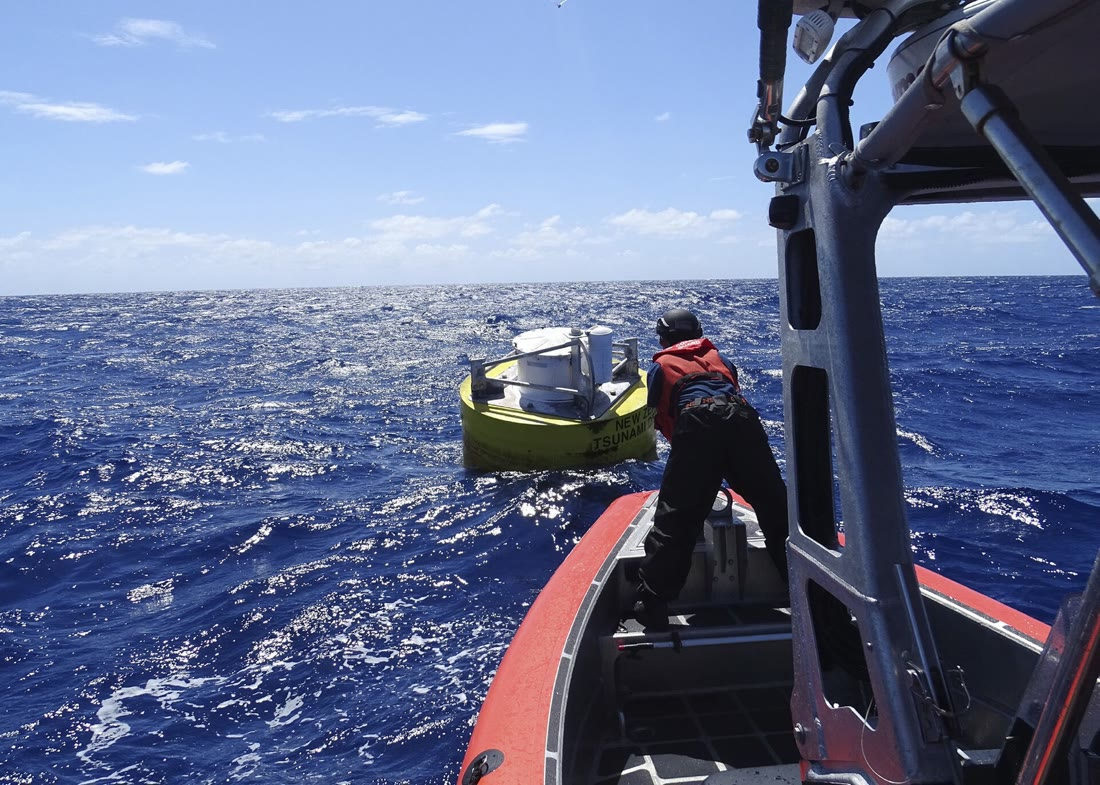
\includegraphics[width=\linewidth]{images/book1/g9-dart-buoy.jpg}
\end{minipage}\hfill
\begin{minipage}[c]{0.56\linewidth}\raggedright
{\small 美国\omterm{def:g1:landscapes-around-us:water}{海岸}警卫队一艘船的一名船员，
于2021年11月在太平洋检查一个\omterm{def:g7:earthquakes:tsunami}{海啸}预警浮标。浮标
漂浮在海底压力计的上方，该压力计位于数千米深的海底。
U.S. Coast Guard（公有领域，经由维基共享资源）。}
\end{minipage}
% ledger: commons:dart-buoy
\label{fig:g9:natural-risks:buoy}
\end{omfigure}

\begin{history}[浮标网络]
2001年，首批由六座此类站点组成的阵列在
太平洋建成。2004年12月的\omterm{def:g7:earthquakes:tsunami}{海啸}抵达
印度洋沿岸，当时尚无预警系统，
（见\cref{ch:g7:earthquakes}），网络不断扩大：到2008年3月，已有
39 个站点。
\end{history}
% ledger: ndbc:dart

预警只有传到懂得如何应对它的人手中，才能挽救生命：通往高处的
路线设有标识并经过演练，应急包已经备好，学校组织演练。
在阿尔梅罗，危害早已为人所知，\omterm{def:g9:natural-risks:hazard-map}{危害分布图}也已绘制，
但预警始终没有传到小镇。
% ledger: ready:kit, usgs:armero

\section{练习}

\begin{exercise}[$\star$]\label{exo:g9:natural-risks:1}
判断下列各项属于危害还是\omterm{def:g9:natural-risks:vulnerability}{脆弱性}？（a）一条几乎每年春季都泛滥的\omterm{def:g1:landscapes-around-us:water}{河流}。
（b）没有预警系统的村庄。（c）用砖砌成、没有框架的厚重房屋。
（d）附近\omterm{def:g7:earthquakes:fault}{断层}上发生的强烈\omterm{def:g4:volcanoes-earthquakes-first-look:earthquake}{地震}。（e）一座城镇建在
曾有泥石流流过的\omterm{def:g1:landscapes-around-us:landform}{山谷}谷口。
\end{exercise}

\begin{exercise}[$\star$]\label{exo:g9:natural-risks:2}
判断下列句子是否正确，并改正错误的句子。（a）无人居住之处的\omterm{def:g5:natural-hazards:hazard}{自然危害}
属于高\omterm{def:g9:natural-risks:risk}{风险}。（b）\omterm{def:g9:natural-risks:prevention}{预防}措施可以降低一座城镇的
\omterm{def:g9:natural-risks:vulnerability}{脆弱性}。（c）\omterm{def:g9:natural-risks:hazard-map}{危害分布图}显示危害可能袭击的地点。
（d）良好的预警系统可使\omterm{def:g4:volcanoes-earthquakes-first-look:volcano}{火山}的危险性降低。
\end{exercise}

\begin{exercise}[$\star$]\label{exo:g9:natural-risks:3}
对每种危害，判断它能否提前数天或数小时预报：
（a）\omterm{def:g5:natural-hazards:storm}{风暴}；（b）大雨后的\omterm{def:g5:water-shapes-the-land:flood}{洪水}；（c）\omterm{def:g4:volcanoes-earthquakes-first-look:earthquake}{地震}；（d）\omterm{def:g7:earthquakes:tsunami}{海啸}
抵达远离其发源地的\omterm{def:g1:landscapes-around-us:water}{海岸}。
\end{exercise}

\begin{exercise}[$\star$]\label{exo:g9:natural-risks:4}
% ledger: usgs:hvo-toolkit
利用一座受监测\omterm{def:g4:volcanoes-earthquakes-first-look:volcano}{火山}的示意图。各仪器测量什么，
它监测的是哪种\omterm{def:g4:volcanoes-earthquakes-first-look:eruption}{喷发}预警信号？（a）\omterm{def:g7:earthquakes:seismometer}{地震仪}。
（b）倾斜仪。（c）GPS 接收机。（d）气体仪器。
\end{exercise}

\begin{exercise}[$\star\star$]\label{exo:g9:natural-risks:5}
% ledger: usgs:armero
1985年，内瓦多德鲁伊斯\omterm{def:g4:volcanoes-earthquakes-first-look:volcano}{火山}的泥石流抵达阿尔梅罗，相距 \qty{45}{km}，
约在\omterm{def:g4:volcanoes-earthquakes-first-look:eruption}{喷发}两小时后到达。（a）它们的平均
速率是多少，以千米每小时为单位？（b）一人步行速度约为
\qty{4}{km/h}。在两小时内，这些人能走多远？
（c）他们为什么没有撤离？（d）请举出两件可能使
他们免于遇难的事。
\end{exercise}

\begin{exercise}[$\star\star$]\label{exo:g9:natural-risks:6}
% ledger: (invented region: figdata/grade-9/flood_zone.py)
利用瓦尔登\omterm{def:g1:landscapes-around-us:landform}{丘陵}的洪泛区图。（a）哪一次\omterm{def:g5:water-shapes-the-land:flood}{洪水}覆盖的
范围最宽？（b）利用图上的网格，测量各\omterm{def:g5:water-shapes-the-land:flood}{洪水}区
在东侧 \qty{5}{km} 处横跨\omterm{def:g1:landscapes-around-us:landform}{山谷}的宽度。（c）一座谷仓位于
河面以上 \qty{6}{m} 的地面上。
三次\omterm{def:g5:water-shapes-the-land:flood}{洪水}中哪几次会淹到它？（d）为何高出河面
\qty{2}{m} 的那次\omterm{def:g5:water-shapes-the-land:flood}{洪水}出现得最频繁？
\end{exercise}

\begin{exercise}[$\star\star$]\label{exo:g9:natural-risks:7}
把每种情形放到\omterm{def:g9:natural-risks:risk}{风险}网格上（危害程度低或高，\omterm{def:g9:natural-risks:vulnerability}{脆弱性}低或高），
并判断\omterm{def:g9:natural-risks:risk}{风险}是低、中等还是高。
（a）位于活动\omterm{def:g7:earthquakes:fault}{断层}上的城镇，建筑坚固并有应急演练。（b）一处
营地位于一条很少泛滥的\omterm{def:g1:landscapes-around-us:water}{河流}的\omterm{def:g5:water-shapes-the-land:flood}{河漫滩}上。（c）一个村庄
由脆弱的房屋组成，位于活\omterm{def:g4:volcanoes-earthquakes-first-look:volcano}{火山}山脚下，且没有观测站。
（d）一座城镇位于山顶，远离任何\omterm{def:g7:earthquakes:fault}{断层}、\omterm{def:g1:landscapes-around-us:water}{河流}或\omterm{def:g4:volcanoes-earthquakes-first-look:volcano}{火山}。
\end{exercise}

\begin{exercise}[$\star\star$]\label{exo:g9:natural-risks:8}
% ledger: iris:better-wall, explo:base-isolation
三所学校建在同一块地面上。A 校为立柱与梁构成的框架，
立柱之间砌有砖墙；B 校框架相同，
但设有斜撑和两道剪力墙；C 校采用 B 校的框架，
但建在隔震支座上。（a）按\omterm{def:g4:volcanoes-earthquakes-first-look:earthquake}{地震}中由最安全到最不安全，为三所学校排序。
（b）说明斜撑的作用。（c）说明
隔震支座的作用。
\end{exercise}

\begin{exercise}[$\star\star$]\label{exo:g9:natural-risks:9}
% ledger: fema:flood-zones
一幅\omterm{def:g5:water-shapes-the-land:flood}{洪水}\omterm{def:g9:natural-risks:risk}{风险}图标出了百年一遇\omterm{def:g5:water-shapes-the-land:flood}{洪水}，它在任一年中被达到或超过的
概率为 1/100。（a）将这一概率写成百分数。
（b）一位邻居说：“百年一遇\omterm{def:g5:water-shapes-the-land:flood}{洪水}去年刚来过，
所以未来 99 年我们都是安全的。”这种说法错在哪里？（c）平均而言，
300 年内会出现多少次这样的\omterm{def:g5:water-shapes-the-land:flood}{洪水}？
\end{exercise}

\begin{exercise}[$\star\star$]\label{exo:g9:natural-risks:10}
% ledger: ndbc:dart, nws:tsunami-speed
\omterm{def:g7:earthquakes:tsunami}{海啸}预警站每隔
\qty{15}{s} 读取一次海底压强。（a）它一小时内记录多少次？（b）在
一个 365 天的年份中呢？结果用科学记数法表示。（c）一次\omterm{def:g7:earthquakes:tsunami}{海啸}
以约 \qty{800}{km/h} 的速度穿过深海。它需要多长时间
才能到达 \qty{2400}{km} 外的\omterm{def:g1:landscapes-around-us:water}{海岸}？（d）这段时间为何重要？
\end{exercise}

\begin{exercise}[$\star\star\star$]\label{exo:g9:natural-risks:11}
% ledger: ready:kit
一家四口准备了应急包，其中有供 3 天使用的水，
按每人每天约 \qty{3.8}{L} 计，用于饮用和洗漱。
（a）他们需要多少升水？（b）这些水相当于多少瓶
\qty{1.5}{L} 的瓶装水？（c）写出应急包中其他四种物品，并
说明每种物品为何有用。（d）应急包为何放在门口附近？
\end{exercise}

\begin{exercise}[$\star\star\star$]\label{exo:g9:natural-risks:12}
% ledger: usgs:armero, usgs:hvo-toolkit
一座城镇位于河边，坐落在一条\omterm{def:g1:landscapes-around-us:landform}{山谷}的谷口，该\omterm{def:g1:landscapes-around-us:landform}{山谷}从一座积雪覆盖的
\omterm{def:g4:volcanoes-earthquakes-first-look:volcano}{火山}延伸而下。城中街道之下埋藏着古老的泥流\omterm{def:g5:water-shapes-the-land:deposition}{沉积}。
\omterm{def:g4:volcanoes-earthquakes-first-look:volcano}{火山}已开始出现小\omterm{def:g4:volcanoes-earthquakes-first-look:earthquake}{地震}。试为该城镇拟定一份
包含五条要点的\omterm{def:g9:natural-risks:prevention}{预防}方案。对每一条，说明它是
作用于危害一侧（认识并监测危害），还是
作用于\omterm{def:g9:natural-risks:risk}{风险}的\omterm{def:g9:natural-risks:vulnerability}{脆弱性}一侧。
\end{exercise}

\section{问题：新学校应建在哪里？}

\begin{problem}[{周末问题——在瓦尔登丘陵的地图上为新学校选址，
远离洪水、陡坡与断层；最终答案是
洪泛区内的房屋数量}]
\label{pb:g9:natural-risks:1}
% ledger: (invented region: figdata/grade-9/flood_zone.py: sites A, B, C; 17 of 28 houses in the 5 m zone)
瓦尔登\omterm{def:g1:landscapes-around-us:landform}{丘陵}的村庄需要一所新学校，拟定了三处候选地点，
分别为 A、B 和 C，见下图。图中阴影所示的洪泛区是
高出河面不足 \qty{5}{m} 的全部地面，一次大\omterm{def:g5:water-shapes-the-land:flood}{洪水}
会淹没这些地面。表格给出了每处地点的
地面高程、河边水位，以及沿坡面水平方向
量取 \qty{200}{m} 时地面的升高量。

\begin{center}
{\small
\begin{tabular}{|c|c|c|c|}
\hline
地点 & 地面高程 & 河边水位 & \qty{200}{m} 内地面升高 \\
\hline
A & \qty{137}{m} & \qty{137}{m} & \qty{1.4}{m} \\
B & \qty{276}{m} & \qty{126}{m} & \qty{83}{m} \\
C & \qty{236}{m} & \qty{143}{m} & \qty{20}{m} \\
\hline
\end{tabular}}
\end{center}

\begin{omfigure}
\begin{tikzpicture}
\begin{axis}[axis equal image, xmin=3.5, xmax=7, ymin=2.7, ymax=5.5, width=11.5cm,
  enlargelimits=false, tick label style={font=\scriptsize}, xlabel={东 (km)},
  ylabel={北 (km)}, label style={font=\small}, xtick={3.5,4,...,7}, ytick={3,3.5,...,5.5}]
\addplot[contour] table {figdata/out/grade-9-flood_zone-contours.dat};
\addplot[index contour] table {figdata/out/grade-9-flood_zone-index.dat};
\addplot[fill=blue!25, draw=blue!50, line width=0.3pt] table {figdata/out/grade-9-flood_zone-zone.dat} -- cycle;
\addplot[only marks, mark=none, point meta=explicit symbolic, nodes near coords,
  nodes near coords align={center}, nodes near coords style={font=\tiny, fill=white, inner sep=0.6pt, text=omContour}]
  table[meta=z] {figdata/out/grade-9-flood_zone-index-lab.dat};
\addplot[river] table {figdata/out/grade-9-flood_zone-river.dat};
\addplot[fault] table {figdata/out/shared-region-fault.dat};
\addplot[only marks, mark=square*, mark size=1.5pt, mark options={fill=black}] table {figdata/out/grade-9-flood_zone-houses-in.dat};
\addplot[only marks, mark=square*, mark size=1.5pt, mark options={fill=black}] table {figdata/out/grade-9-flood_zone-houses-out.dat};
\addplot[only marks, mark=*, mark size=2.6pt, mark options={fill=omWarm, draw=black}, point meta=explicit symbolic, nodes near coords align={anchor=south west}]
  table[meta=name] {figdata/out/grade-9-flood_zone-sites.dat};
\node[font=\small\bfseries, fill=white, inner sep=1pt, xshift=2.5pt, yshift=2.5pt, anchor=south] at (axis cs:4.7,3.5316) {A};
\node[font=\small\bfseries, fill=white, inner sep=1pt, xshift=2.5pt, yshift=2.5pt, anchor=south] at (axis cs:6.3,4.4473) {B};
\node[font=\small\bfseries, fill=white, inner sep=1pt, xshift=2.5pt, yshift=2.5pt, anchor=south] at (axis cs:3.8,2.8404) {C};
\node[font=\footnotesize, fill=white, inner sep=1pt, anchor=west] at (axis cs:6.42,5.05) {断层};
\coordinate (na) at (axis cs:3.7,4.75);
\fill[black] (axis cs:5.8,2.85) rectangle (axis cs:5.925,2.9);
\fill[white] (axis cs:5.925,2.85) rectangle (axis cs:6.05,2.9);
\fill[black] (axis cs:6.05,2.85) rectangle (axis cs:6.175,2.9);
\fill[white] (axis cs:6.175,2.85) rectangle (axis cs:6.3,2.9);
\draw[black, line width=0.4pt] (axis cs:5.8,2.85) rectangle (axis cs:6.3,2.9);
\node[font=\footnotesize, above, inner sep=1.5pt, fill=white] at (axis cs:6.05,2.9) {\qty{500}{m}};
\end{axis}
\fill[white, opacity=0.85] ($(na)+(-0.35,-0.1)$) rectangle ($(na)+(0.35,1.45)$);
\pic at (na) {northarrow};
\end{tikzpicture}

{\small 村庄、三处学校选址及洪泛区（阴影部分），
在瓦尔登\omterm{def:g1:landscapes-around-us:landform}{丘陵}\omterm{def:g2:drawing-to-map:map}{地图}上（细线为等高线，每
\qty{10}{m}）。每个小黑方块代表一座房屋。粗黑线
为\omterm{def:g7:earthquakes:fault}{断层}。}
\label{fig:g9:natural-risks:school-map}
\end{omfigure}

\noindent\textbf{第一部分——洪泛区。}\par\nopagebreak
\begin{enumerate}[beginpenalty=10000]
  \item 根据表中\omterm{def:g1:landscapes-around-us:water}{河流}水位数据，
        判断河水流向。
  \item 计算每处选址相对于其旁\omterm{def:g1:landscapes-around-us:water}{河流}的高度。
  \item 三处选址中，哪一处位于洪泛区？
  \item 利用线段\omterm{def:g2:drawing-to-map:scale}{比例尺}，测量A处洪泛区的宽度，
        即横跨\omterm{def:g1:landscapes-around-us:landform}{山谷}的距离。
\end{enumerate}

\noindent\textbf{第二部分——坡度与\omterm{def:g7:earthquakes:fault}{断层}。}\par\nopagebreak
\begin{enumerate}[resume, beginpenalty=10000]
  \item 坡度以百分数表示，即水平距离每
        \qty{100}{m}内地面上升的高度。计算各选址处的坡度。
  \item 哪一处选址最易遭受\omterm{def:g5:natural-hazards:landslide}{滑坡}？请说明理由。
  \item 利用线段\omterm{def:g2:drawing-to-map:scale}{比例尺}，估算各选址到
        \omterm{def:g7:earthquakes:fault}{断层}的距离。
  \item 假设该\omterm{def:g7:earthquakes:fault}{断层}仍可能活动。为什么\omterm{def:g7:earthquakes:fault}{断层}正上方的
        地面不适合建造学校？
\end{enumerate}

\noindent\textbf{第三部分——选址。}\par\nopagebreak
\begin{enumerate}[resume, beginpenalty=10000]
  \item 画一张表格，每个选址占一行，设三列：
        是否位于洪泛区？是否为陡坡？是否位于\omterm{def:g7:earthquakes:fault}{断层}上？用“是”或“否”填写。
  \item 你会选择哪一处？请结合表格说明理由。
  \item 所选选址仍位于地面可能发生震动的
        地区。请说出两种学校建造方式和学生的一种习惯，
        以降低学校的\omterm{def:g9:natural-risks:vulnerability}{脆弱性}。
  \item 该学校在\omterm{def:g5:water-shapes-the-land:flood}{洪水}期间还将用作避难所。统计
        村庄中位于洪泛区内的房屋数量，
        这占全部房屋的比例是多少？
\end{enumerate}
\end{problem}
